% Options for packages loaded elsewhere
\PassOptionsToPackage{unicode}{hyperref}
\PassOptionsToPackage{hyphens}{url}
\PassOptionsToPackage{dvipsnames,svgnames,x11names}{xcolor}
%
\documentclass[
  10pt,
]{article}
\usepackage{amsmath,amssymb}
\usepackage{iftex}
\ifPDFTeX
  \usepackage[T1]{fontenc}
  \usepackage[utf8]{inputenc}
  \usepackage{textcomp} % provide euro and other symbols
\else % if luatex or xetex
  \usepackage{unicode-math} % this also loads fontspec
  \defaultfontfeatures{Scale=MatchLowercase}
  \defaultfontfeatures[\rmfamily]{Ligatures=TeX,Scale=1}
\fi
\usepackage{lmodern}
\ifPDFTeX\else
  % xetex/luatex font selection
  \setmainfont[]{DejaVu Serif}
  \setsansfont[]{DejaVu Sans}
  \setmonofont[]{DejaVu Sans Mono}
\fi
% Use upquote if available, for straight quotes in verbatim environments
\IfFileExists{upquote.sty}{\usepackage{upquote}}{}
\IfFileExists{microtype.sty}{% use microtype if available
  \usepackage[]{microtype}
  \UseMicrotypeSet[protrusion]{basicmath} % disable protrusion for tt fonts
}{}
\makeatletter
\@ifundefined{KOMAClassName}{% if non-KOMA class
  \IfFileExists{parskip.sty}{%
    \usepackage{parskip}
  }{% else
    \setlength{\parindent}{0pt}
    \setlength{\parskip}{6pt plus 2pt minus 1pt}}
}{% if KOMA class
  \KOMAoptions{parskip=half}}
\makeatother
\usepackage{xcolor}
\usepackage[margin=22mm]{geometry}
\usepackage{longtable,booktabs,array}
\usepackage{calc} % for calculating minipage widths
% Correct order of tables after \paragraph or \subparagraph
\usepackage{etoolbox}
\makeatletter
\patchcmd\longtable{\par}{\if@noskipsec\mbox{}\fi\par}{}{}
\makeatother
% Allow footnotes in longtable head/foot
\IfFileExists{footnotehyper.sty}{\usepackage{footnotehyper}}{\usepackage{footnote}}
\makesavenoteenv{longtable}
\usepackage{graphicx}
\makeatletter
\def\maxwidth{\ifdim\Gin@nat@width>\linewidth\linewidth\else\Gin@nat@width\fi}
\def\maxheight{\ifdim\Gin@nat@height>\textheight\textheight\else\Gin@nat@height\fi}
\makeatother
% Scale images if necessary, so that they will not overflow the page
% margins by default, and it is still possible to overwrite the defaults
% using explicit options in \includegraphics[width, height, ...]{}
\setkeys{Gin}{width=\maxwidth,height=\maxheight,keepaspectratio}
% Set default figure placement to htbp
\makeatletter
\def\fps@figure{htbp}
\makeatother
\setlength{\emergencystretch}{3em} % prevent overfull lines
\providecommand{\tightlist}{%
  \setlength{\itemsep}{0pt}\setlength{\parskip}{0pt}}
\setcounter{secnumdepth}{-\maxdimen} % remove section numbering
\ifLuaTeX
  \usepackage{selnolig}  % disable illegal ligatures
\fi
\IfFileExists{bookmark.sty}{\usepackage{bookmark}}{\usepackage{hyperref}}
\IfFileExists{xurl.sty}{\usepackage{xurl}}{} % add URL line breaks if available
\urlstyle{same}
\hypersetup{
  pdftitle={Stage 0: From angular structure to conditional kinematic constraints},
  colorlinks=true,
  linkcolor={Maroon},
  filecolor={Maroon},
  citecolor={Blue},
  urlcolor={Blue},
  pdfcreator={LaTeX via pandoc}}

\title{Stage 0: From angular structure to conditional kinematic
constraints}
\usepackage{etoolbox}
\makeatletter
\providecommand{\subtitle}[1]{% add subtitle to \maketitle
  \apptocmd{\@title}{\par {\large #1 \par}}{}{}
}
\makeatother
\subtitle{A converged baseline from radiation, astrometry, optical
distances and finite geometry images}
\author{}
\date{28 October 2026}

\begin{document}
\maketitle

\hypertarget{physical-question-and-common-representation}{%
\section{Physical question and common
representation}\label{physical-question-and-common-representation}}

\textbf{Scope at uptake.} This Stage 0 report reuses qualified finite
and observational products; it adds no catalogue fit, native low-ell
transfer, ODE evolution, or original scientific acceptance. The original
external-output ledger remains \textbf{17/42}; a separate analytic
alternate records \textbf{18/42} and does not replace the V03
external-history obligation. PR4/P2 manuscript preparation is
\textbf{PREPARED\_PENDING\_SOURCE\_QUALIFICATION}, with no actual MC100
approval. Every number below is interpreted at the source's stated law
and target. A correctly specified common-response carrier and joint GLS
have equal information under the same full law; compression is valuable
for retaining, rather than increasing, information.

Angular structure becomes a constraint on spacetime only after its
response to a specified physical state is identified. A temperature
multipole, an apparent-magnitude quadrupole and an astrometric electric
quadrupole are different observables. Their tensor representations can
preserve orientation and sign, but their physical meanings follow from
radiative transfer, optical propagation and source motion. The common
inference problem is therefore

\[
Y=\mathscr R_\eta(X_{\rm phys})+\epsilon,
\qquad
\mathcal K(Y)=\{\theta:\mathscr R_\eta(\theta)\text{ is compatible with }Y
\text{ for an admitted }\eta\}.
\]

Here \(\eta\) contains physical histories, processing and calibration
variables appropriate to the observation. A compatibility region can
constrain a named combination even when the individual parameters remain
degenerate. The present results connect retained observations and finite
response calculations to four targets: radiation-to-kinematics,
beyond-FLRW kinematic quantities, physical-family classification, and
direction/redshift-dependent expansion.

The five coordinates \((x,F,Q,\Pi,G_F)\) organize these calculations
without changing the observational law. The carrier \(x\) retains signed
coefficients, their representation, frame and units. For a physical
image \(\mathcal C\), \(F(W)=\sup_{x\in\mathcal C}\langle W,x\rangle\)
measures its extent in a declared direction. A gauge \(Q\) measures
displacement relative to a specified centred reference body; a positive
cone or an uncentred trace-one slice is not automatically a usable gauge
body. \(\Pi\) records probability only under the declared sampling or
posterior law. \(G_F\) retains the comparison maps and cross-window
dependence needed to follow the same object through depth or transport.
Nonconvex family labels remain attached to their images because a
support function alone records their convex hull.

This distinction is operational. In the saved Gaussian-carrier
comparison, tensorized and correctly specified joint GLS estimates
agreed to a maximum absolute difference of \(2.42\times10^{-13}\), and
their information matrices to \(2.15\times10^{-16}\). A common
response-family carrier had dimension 12, whereas a single-family
carrier had dimension 6. The former retained the compared likelihood
ratios; the latter could erase their discrimination. These are fixed-law
compression results, with the physical response held constant {[}E1{]}.

A supplied approximation bound can be transported through the same
structure. If \(e^TGe\le\epsilon_X^2\) and its observation response is
\(b=Be\), then

\[
\sup_e v^TBe=\epsilon_X\sqrt{v^TBG^{-1}B^Tv}.
\]

The matrix in this expression describes a deterministic joint error
body. Keeping its shared directions can be substantially sharper than
bounding each observable separately. After nuisance projection, this
body induces a bound on parameter bias and a corresponding confidence
region. In a finite five-parameter Gaussian control with bias radius 1.5
in Fisher units, the ordinary nominal 95\% ball had exact coverage
82.7209\%; the bias-aware construction had exact coverage 95\% and Monte
Carlo coverage 95.098\% in 100,000 draws {[}E2{]}. The physical
significance is that truncation or response error enters the inferential
region instead of disappearing behind a small statistical error bar.

\begin{figure}
\centering
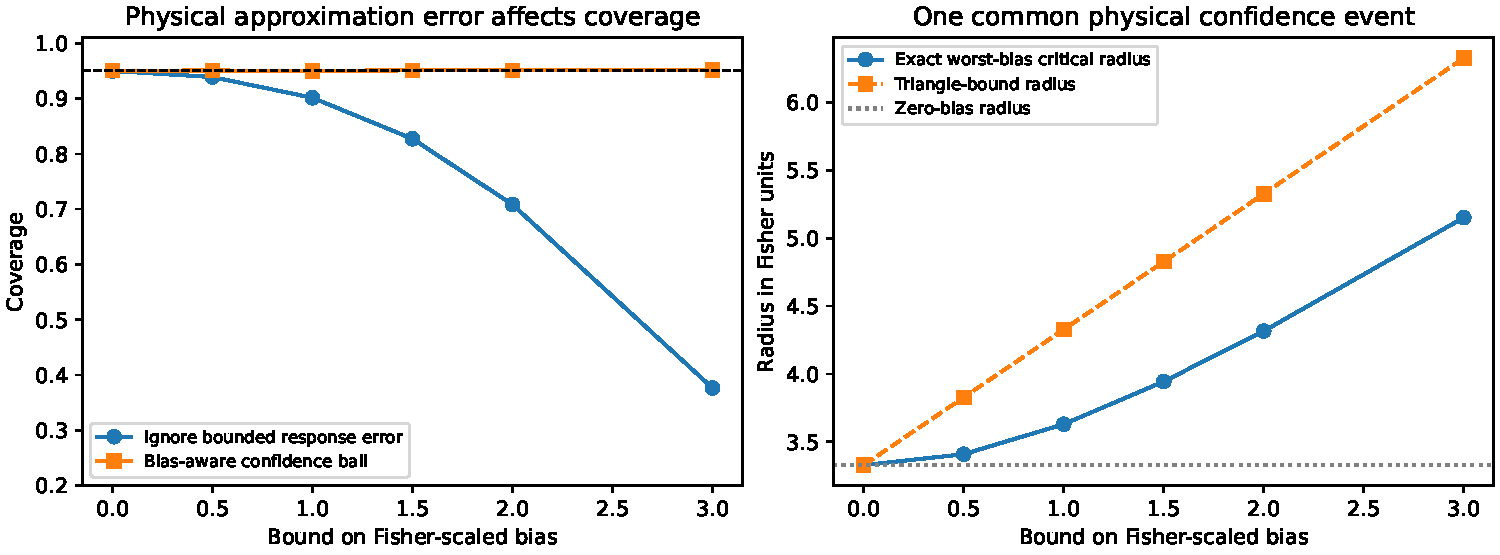
\includegraphics[width=1\textwidth,height=\textheight]{../../imports/four_goals/figures/joint_remainder.pdf}
\caption{A common physical error bound propagated to parameter coverage,
compared with ignoring the bounded bias.}
\end{figure}

Internal polarization illustrates the same distinction at the detector
level. The positive distribution
\(f=f_0[I+(n\cdot e)\theta\cdot\sigma]\), \(\|\theta\|\le1\), can
preserve total trace and stress while retaining opposite channel
currents. In the executed finite count experiment, calibrated channel
data distinguished two opposite-sign states with 98.086\% accuracy in
100,000 equal-prior trials; trace or sorted state spectra gave 50\%.
Known zero calibration allowed three pooled sufficient counts, whereas
an unknown common calibration required the six-channel natural-parameter
span {[}E12{]}. This is an information statement for the specified count
law. A geometric helicity phase connection and a physical polarization
converter have different measurement spans and are kept distinct.

\hypertarget{low-multipole-morphology-and-the-radiation-to-shear-response}{%
\section{1. Low-multipole morphology and the radiation-to-shear
response}\label{low-multipole-morphology-and-the-radiation-to-shear-response}}

The local radiation field carries an energy density, flux and
anisotropic stress. For a complete blackbody temperature sky the
bolometric intensity is proportional to \(T^4\), so a linear
temperature-to-stress conversion need not preserve the finite physical
target. This has already been tested using the same positive synthetic
skies and correlated temperature errors for both adapters. In the
isotropic-rest-frame case with observer speed \(\beta=0.00123\), the
exact adapter's radiative tensor target had 94.531\% coverage, while the
linear adapter had 74.097\%. The scalar rest-frame stress-anisotropy
target had 95.557\% versus 37.720\% coverage. At \(\beta=0.3\), the
corresponding exact coverages were 96.045\% and 95.386\%, while both
linear physical-target coverages were zero. Each case used 8,191
calibration skies and 4,096 independent test skies {[}E3{]}.

The tensor target is the finite-boost stress residual \[
\mathscr D=\frac\pi\rho-k_\gamma(f\cdot f)\operatorname{STF}(f\otimes f),
\qquad f=\frac{q}{c\rho},\qquad
k_\gamma(s)=\frac3{2+\sqrt{4-3s}}.
\] It tests whether the measured energy flux and anisotropic stress have
the relation induced by a boosted isotropic radiation stress tensor. The
companion scalar is the norm of the Landau-frame pressure departures
from \(\rho_L/3\), divided by \(\rho_L\). These stress-level targets
distinguish observer-induced dipole structure from a residual rest-frame
anisotropic stress; they do not replace the higher-multipole
distribution or the spacetime response.

The linear method remained calibrated for its own approximate target.
Its loss concerned the physical quantity to which that target was being
assigned. This provides a concrete reason to retain the physical
response map through inference. It also separates a response bias from a
failure of a numerical likelihood algorithm.

\begin{figure}
\centering
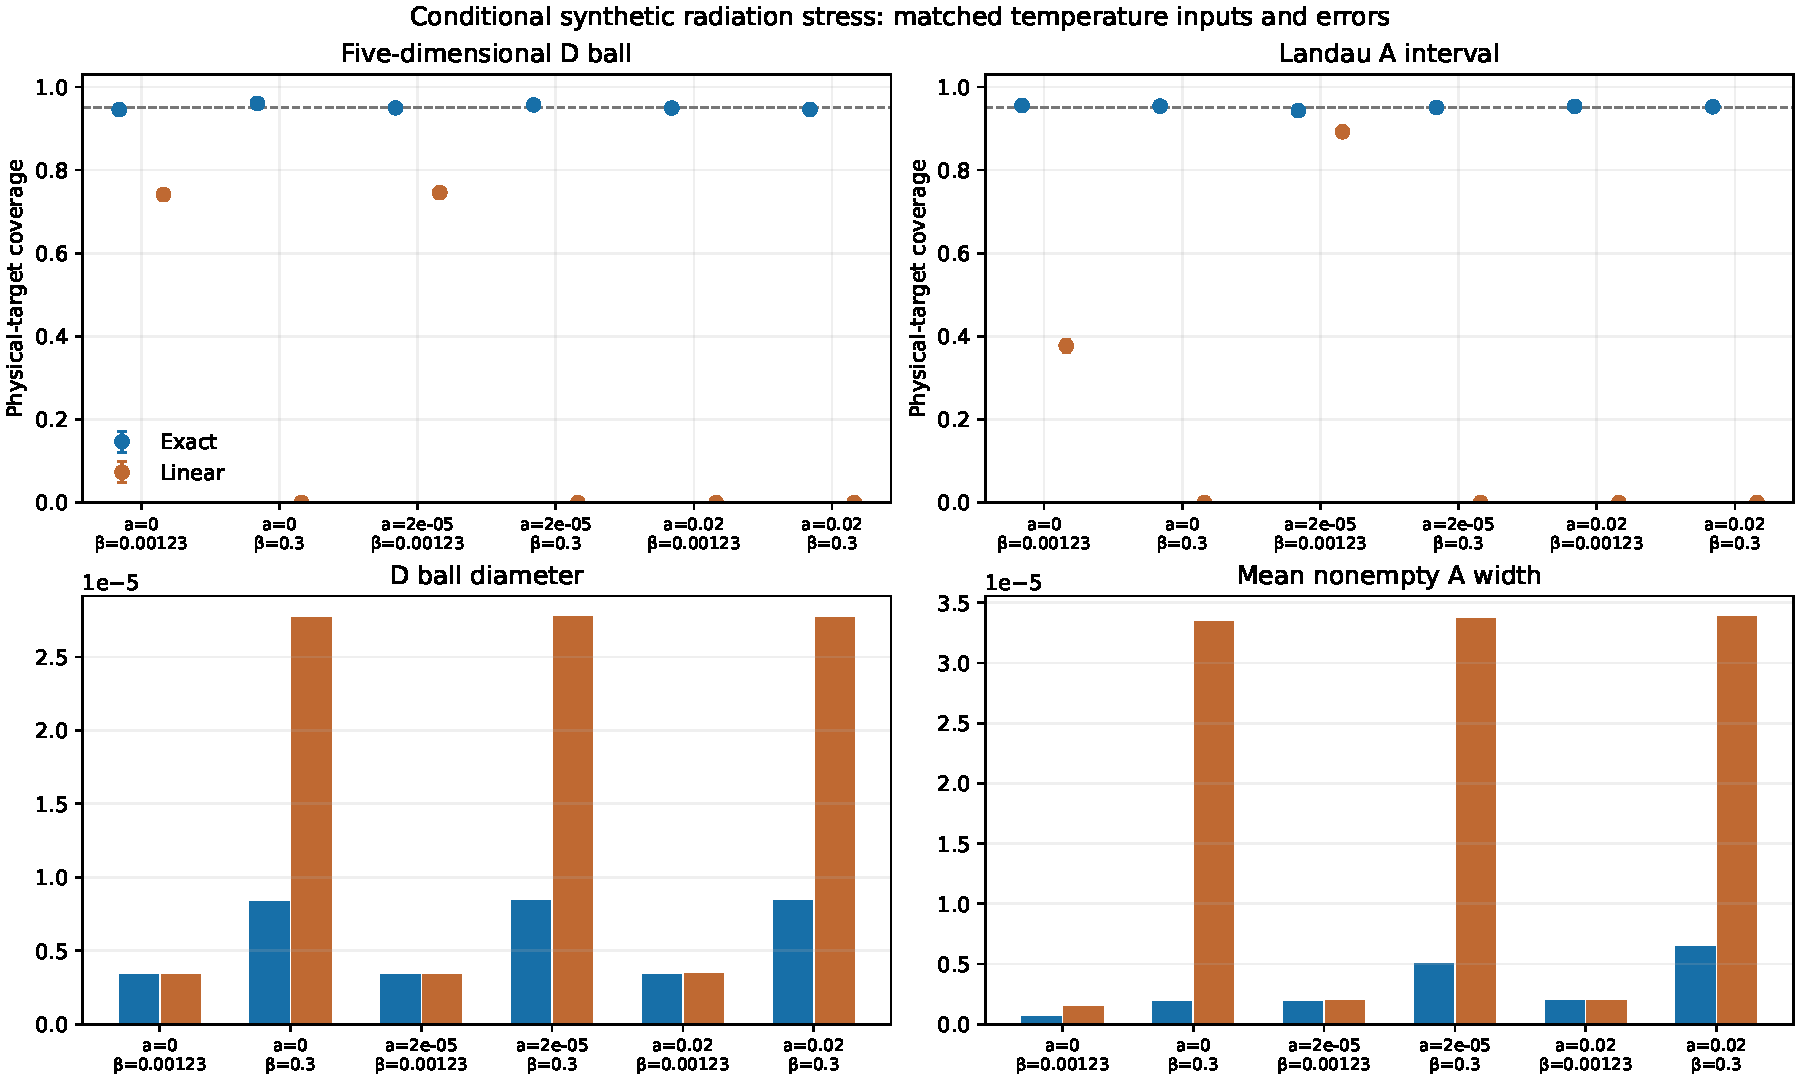
\includegraphics[width=1\textwidth,height=\textheight]{../../../OBSERVABLE_BRIDGE_RECONCILIATION_20261027/products/R36-05-RADIATION-RESPONSE/comparison.pdf}
\caption{Common-input radiation comparison: exact and linear
temperature-to-stress adapters under the same finite synthetic law.}
\end{figure}

The instantaneous shear-response operator \(\mathcal L_I\) acts on the
five-dimensional STF shear space. Its complete angular dependence is
determined by intensity moments of degrees 0, 2 and 4. In the retained
positive-sky compression test, truncation at degree 2 changed the
operator by \(0.00654243536\,\rho_0\) in operator norm. Retaining degree
4 reduced that discrepancy to \(3.34\times10^{-16}\,\rho_0\) at the
primary quadrature, although higher angular information remained
unresolved {[}E3{]}. Moment completeness is therefore relative to the
response being computed.

Polarization introduces a second response to preserve. For cold-electron
Thomson gain in a fixed electron frame, let \(\mathsf F(n)\) be the
transverse polarization matrix, \(P_n=I-nn^T\), and
\(M=\int\mathsf F(n)\,d\Omega\). The gain is

\[
\mathscr G\mathsf F(n)=\frac{3}{8\pi}P_nMP_n.
\]

Its finite Hermitian carrier determines the gain, while the full
collision operator also retains the incident-field loss. The positive
intensity fields \(I_\pm=1\pm0.6P_4(n_z)\) have identical gain but
different shear operators. Their global intensity lower bound is 0.4,
and the computed operator separation is 0.5744626567 in the example's
normalization {[}E4{]}. A compression sufficient for gain is
consequently insufficient for the joint gain-and-shear question.

Near the positive unpolarized reference, the joint linear carrier can be
written

\[
x_{\rm rad}=(\rho,\pi,H_4,P_*,A_*),
\qquad \dim x_{\rm rad}=1+5+9+5+3=23.
\]

Here \(P_*\) is the integrated linear-polarization STF contribution and
\(A_*\) the circular sector. Excluding a circular target leaves
dimension 20. Exact rational angular-moment checks independently
confirmed these ranks {[}E4{]}. They specify what to preserve for these
outputs, rather than requiring the full angular field for every
subsequent question.

The same calculation makes the physical consequence of polarization
omission explicit:

\[
C_\pi=-\gamma_T\left(\frac9{10}\pi+\frac15P_*\right),
\qquad
\Sigma_{\rm true}-\Sigma_{\rm unpol}
=-\frac{\gamma_T}{5}\mathcal L_I^{-1}P_*.
\]

For a positive invertible \(\mathcal L_I\), this gives
\(\|\Delta\Sigma\|\le\gamma_T\|P_*\|/[5\lambda_{\min}(\mathcal L_I)]\).
The finite positive-screen example attained a bias and bound of 0.0072
in its declared toy time units {[}E4{]}. The measurable radiation
moments specify the operator; the transport derivative/collision
residual specifies the right-hand side of the conditional shear inverse.
This is the precise place at which a physical history assumption enters.

The next refinement is a directional shear-support plot against the
supplied residual allowance, comparing full and reduced responses on
identical T/Q/U inputs. The existing result is already a complete
conditional response calculation. A Planck application must add the
measured channel, spectral, beam/mask and joint-error definitions before
giving that plot an observational interpretation.

\hypertarget{kinematic-quantities-from-optical-and-transverse-responses}{%
\section{2. Kinematic quantities from optical and transverse
responses}\label{kinematic-quantities-from-optical-and-transverse-responses}}

For one specified smooth congruence, the local longitudinal expansion is

\[
\mathcal H_u(n)=H-\frac{A\cdot n}{c}+\sigma:nn
=H(1+d\cdot n+S:nn),
\quad d=-\frac{A}{cH},\quad S=\frac\sigma H.
\]

The antisymmetric velocity gradient drops out of this contraction.
Nevertheless, nonlinear optical observables retain informative
couplings. With \(\kappa=5/\ln10\), the intercept-subtracted magnitude
field is \(-\kappa\log(1+d\cdot n+S:nn)\). Its STF octupole obeys

\[
O_\mu=\kappa L_Sd+R_3,
\quad L_Sd=\operatorname{STF}(d\otimes S),
\quad L_S^TL_S=\frac{S:S}{3}I+\frac25S^2.
\]

The direct dipole, quadrupole and octupole therefore provide a joint
compatibility test of a physical response. The retained source-level
calculation pushes the full covariance through \([ -\kappa L_S,I_7]\)
and uses one remainder budget for all seven octupole coordinates. A
finite counterexample has perpendicular and parallel normalized
residuals of 0.8 each: both separate checks pass, while their combined
norm is \(\sqrt{1.28}=1.13137\) and fails the common unit budget
{[}E5{]}. The test constrains the stated response/error class; its
failure does not identify one unique astrophysical cause.

Transverse information supplies a complementary projection. For a
spatial gradient \(K\), define \(H(n)=n^TKn\) and \(Q(n)=P_nKn\). Then

\[
K=3\left\langle[nH(n)+Q(n)]n^T\right\rangle_{S^2}.
\]

In the ideal Hermitian two-channel extension, combining a full internal
detector span with radial and transverse responses identifies 36 real
gradient components. Free common catalogue spin removes three geometric
vorticity directions, leaving rank 33. These are calibrated response
ranks; a polarimetric flux measurement supplies a gradient component
only through its actual source/detector map {[}E6{]}.

The selected Gaia field gives an observationally anchored example of
this separation. The retained normal equations encode 755,850 selected
rows and all cross terms between the common electric quadrupole and
nuisance coefficients. Under the reported marginal proper-motion errors
and stipulated cross-source independence, both the six-common-spin/glide
fit and the all-97-nuisance fit retain five electric-quadrupole
directions. Their signed STF coefficients, in
\(\mu\mathrm{as}\,\mathrm{yr}^{-1}\), are {[}E7{]}:

\begin{longtable}[]{@{}
  >{\raggedright\arraybackslash}p{(\columnwidth - 10\tabcolsep) * \real{0.1667}}
  >{\raggedleft\arraybackslash}p{(\columnwidth - 10\tabcolsep) * \real{0.1667}}
  >{\raggedleft\arraybackslash}p{(\columnwidth - 10\tabcolsep) * \real{0.1667}}
  >{\raggedleft\arraybackslash}p{(\columnwidth - 10\tabcolsep) * \real{0.1667}}
  >{\raggedleft\arraybackslash}p{(\columnwidth - 10\tabcolsep) * \real{0.1667}}
  >{\raggedleft\arraybackslash}p{(\columnwidth - 10\tabcolsep) * \real{0.1667}}@{}}
\toprule\noalign{}
\begin{minipage}[b]{\linewidth}\raggedright
Nuisance treatment
\end{minipage} & \begin{minipage}[b]{\linewidth}\raggedleft
STF 1
\end{minipage} & \begin{minipage}[b]{\linewidth}\raggedleft
STF 2
\end{minipage} & \begin{minipage}[b]{\linewidth}\raggedleft
STF 3
\end{minipage} & \begin{minipage}[b]{\linewidth}\raggedleft
STF 4
\end{minipage} & \begin{minipage}[b]{\linewidth}\raggedleft
STF 5
\end{minipage} \\
\midrule\noalign{}
\endhead
\bottomrule\noalign{}
\endlastfoot
Six common spin/glide terms & -2.2624 & 2.2718 & -3.6530 & -2.7187 &
2.3952 \\
All 97 retained nuisance terms & -5.7272 & 1.1566 & -7.4275 & -5.5617 &
6.1770 \\
\end{longtable}

The two rows describe the same selected data under different nuisance
projections. Their change is a direct demonstration of the role of the
shared field and covariance. The primary working-law 80\%-power radii
range from 1.60963 to 2.29431 \(\mu\mathrm{as}\,\mathrm{yr}^{-1}\) along
its information eigenvectors {[}E7{]}. They quantify the design's
sensitivity to a common response tensor, not a calibrated matter-shear
measurement.

For comoving sources and observer in the declared weak fixed-axis
homogeneous geometry, that response is

\[
\mu(n)=P_n\mathcal A n,
\qquad
\mathcal A=\frac{2c(B_o-B_s)}D-\dot B_o.
\]

The nearby limit gives \(\mathcal A\simeq\sigma_o\), while a negligible
endpoint term gives \(-\sigma_o\). The measured sign therefore has
history-dependent meaning. In the common-distance parameterization
\(\mathcal A=kq-s\), the ten endpoint/derivative coordinates have a
five-dimensional observable image and the null direction
\(\delta s=k\delta q\). Keeping both endpoint and derivative quantities
makes that degeneracy explicit rather than silently assigning the same
angular field to one physical tensor.

\begin{figure}
\centering
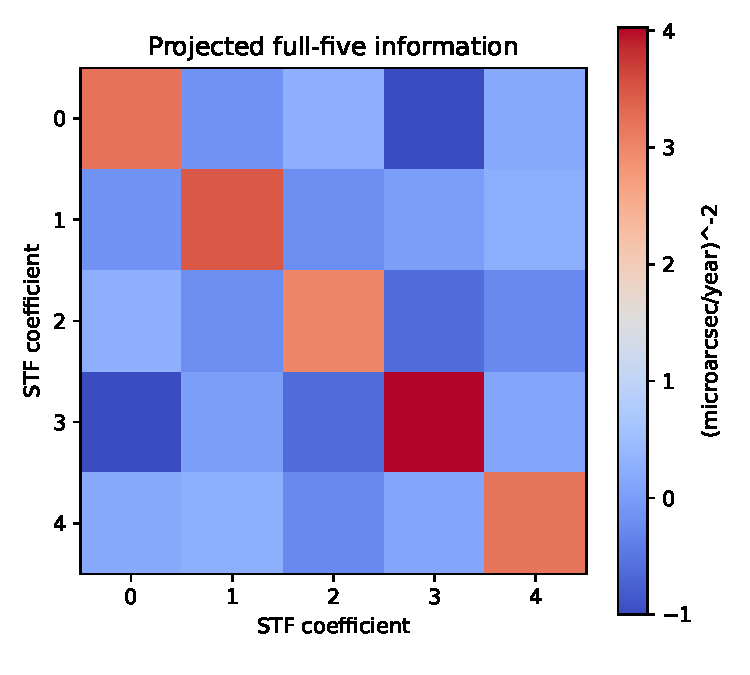
\includegraphics[width=1\textwidth,height=\textheight]{../../../OBSERVABLE_BRIDGE_RECONCILIATION_20261027/products/R36-03-PM-HISTORY/INFORMATION.pdf}
\caption{Selected-sample proper-motion information for the common STF
response, with nuisance dependence retained.}
\end{figure}

The next refinement propagates a supplied finite-history/optical
remainder through these retained normal equations and displays the
resulting physical image. It reuses the measured signed field and full
cross blocks without inventing new source-dependent depth moments.

\hypertarget{physical-family-comparison-and-geometric-stability}{%
\section{3. Physical-family comparison and geometric
stability}\label{physical-family-comparison-and-geometric-stability}}

Kinematics contributes to geometry through field equations and
constraints. For a hypersurface-normal congruence, write \(h=H/c\),
\(S=\sigma/c\), and \(\kappa_g=8\pi G/c^4\). The relevant Gauss
relations are

\[
{}^3R=2\kappa_g\rho+2\Lambda-6h^2+S:S,
\] \[
{}^3R_{\langle ij\rangle}
=E_{ij}+\frac{\kappa_g}{2}\pi_{ij}-hS_{ij}
+\operatorname{STF}(S^2)_{ij}.
\]

The electric-Weyl and anisotropic-stress terms show what additional
physics is required to turn a shear image into a curvature image. A
tensor classification can then compare supplied physical families after
orientation, nuisance and approximation error have been included.

The retained type-II and unequal-VII0 finite witnesses have sorted Ricci
spectra \((-1/2,-1/2,1/2)u_*^2\) and \((-3/2,-1/2,3/2)u_*^2\). Their
scalar curvatures are both \(-u_*^2/2\), but their rotation-orbit
separation is \(\sqrt2u_*^2\). Their quadratic curvature invariants are
\(3u_*^4/4\) and \(19u_*^4/4\), so a suitable scalar invariant also
distinguishes this noiseless pair {[}E8{]}. The physical advantage of
retaining the tensor is the controlled joint response and uncertainty
calculation, not an assertion that every scalar is inadequate.

For family images \(\mathcal M_k\), a common confidence ball of radius
\(r_\alpha\) and physical approximation radii \(\epsilon_k\) gives

\[
\widehat{\mathcal K}_\alpha
=\{k:\operatorname{dist}(z,\mathcal M_k)\le r_\alpha+\epsilon_k\}.
\]

The sufficient separation condition is
\(\operatorname{dist}(\mathcal M_k,\mathcal M_l)>2r_\alpha+\epsilon_k+\epsilon_l\).
In the executed Gaussian geometry-response example, the common
likelihood-ratio carrier has five STF coordinates; a sixth trace
direction remains useful for detecting that both listed families are
inadequate {[}E8{]}. This complements classification with a test of the
family list itself. Near the FLRW limit, overlapping physical images
naturally yield multiple compatible labels.

\begin{figure}
\centering
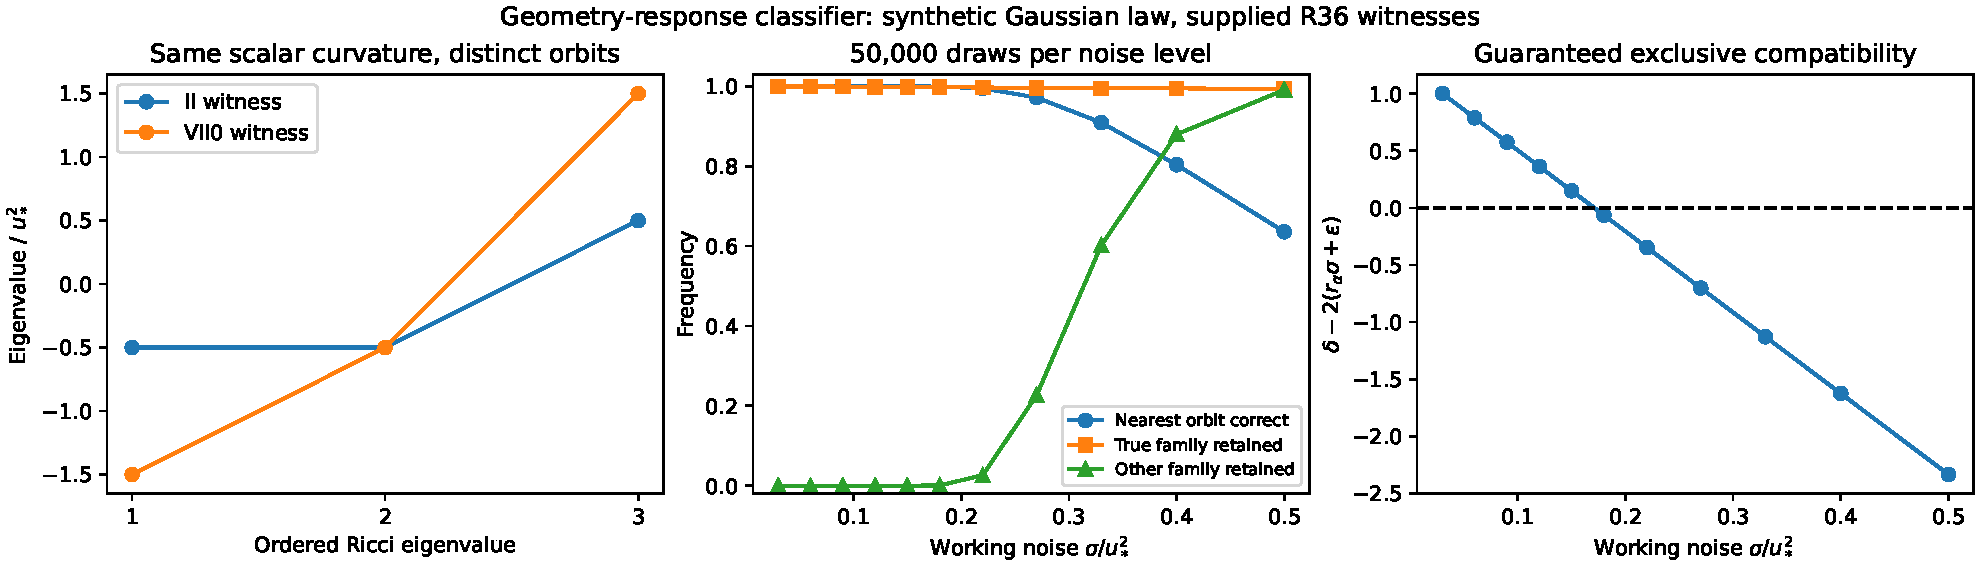
\includegraphics[width=1\textwidth,height=\textheight]{../../imports/four_goals/figures/goal3_classification.pdf}
\caption{Finite geometry-response classification: equal scalar
curvature, separated tensor orbits, and compatibility as the error
budget changes.}
\end{figure}

Morphological stability has an exact local formulation as well. For
fixed simple-spectrum quadrupole \(Q\), let \(v=O:Q\), \(t=Q:Q\), and
\(m_i=t/3+2\lambda_i^2/5\) in its eigenbasis. The distance in ambient
STF3 Frobenius norm to a zero-chirality surface is

\[
\rho_{\rm sign}=\min_i\frac{|v_i|}{\sqrt{m_i}}.
\]

The retained sharp witness attains \(1/\sqrt3\); an independently
constructed boundary perturbation makes chirality vanish to numerical
precision {[}E8{]}. This turns a chosen perturbation-radius test into a
radius tied to the actual sign-changing geometry. Uncertainty in \(Q\)
requires its own joint image rather than substituting a point estimate
into the fixed-Q theorem.

The next refinement is a common-confidence comparison of already
supplied geometry or PM-history families, including the adequacy
residual. CMB Bianchi labels enter through full, source-qualified
temperature/polarization family responses with their histories and
processing conventions.

\hypertarget{directional-expansion-and-optical-transmission}{%
\section{4. Directional expansion and optical
transmission}\label{directional-expansion-and-optical-transmission}}

The released supernova magnitude field already supplies a concrete
signed angular result. The primary Pantheon+ sample excludes calibrators
and uses \(0.0233\le z_{\rm HD}\le0.15\), split at 0.06. A global
intercept and one depth offset are profiled. Dipole and STF-quadrupole
terms in each bin give a 16-coordinate angular carrier. The released
STAT+SYS covariance is used once, retaining cross-depth terms {[}E9{]}.

\begin{longtable}[]{@{}
  >{\raggedright\arraybackslash}p{(\columnwidth - 10\tabcolsep) * \real{0.1667}}
  >{\raggedleft\arraybackslash}p{(\columnwidth - 10\tabcolsep) * \real{0.1667}}
  >{\raggedleft\arraybackslash}p{(\columnwidth - 10\tabcolsep) * \real{0.1667}}
  >{\raggedleft\arraybackslash}p{(\columnwidth - 10\tabcolsep) * \real{0.1667}}
  >{\raggedleft\arraybackslash}p{(\columnwidth - 10\tabcolsep) * \real{0.1667}}
  >{\raggedleft\arraybackslash}p{(\columnwidth - 10\tabcolsep) * \real{0.1667}}@{}}
\toprule\noalign{}
\begin{minipage}[b]{\linewidth}\raggedright
Cohort
\end{minipage} & \begin{minipage}[b]{\linewidth}\raggedleft
Low/high rows
\end{minipage} & \begin{minipage}[b]{\linewidth}\raggedleft
Isotropic residual statistic
\end{minipage} & \begin{minipage}[b]{\linewidth}\raggedleft
Angular residual statistic
\end{minipage} & \begin{minipage}[b]{\linewidth}\raggedleft
Improvement
\end{minipage} & \begin{minipage}[b]{\linewidth}\raggedleft
Conditional upper-tail probability
\end{minipage} \\
\midrule\noalign{}
\endhead
\bottomrule\noalign{}
\endlastfoot
Primary & 342 / 148 & 433.4585 & 416.2519 & 17.2066 & 0.37235 \\
Lower-redshift sensitivity & 557 / 148 & 608.5020 & 591.9479 & 16.5541 &
0.41500 \\
\end{longtable}

Under the stipulated fixed-design Gaussian law, the angular improvement
is below the 5\% \(\chi^2_{16}\) threshold of 26.2962 in both
overlapping cohorts. The primary dipoles are
\((0.01758,0.03002,0.01848)\) mag at low depth and
\((0.00223,0.02426,0.05879)\) mag at high depth. The full signed vector
and its covariance retain how these angular patterns change together
{[}E9{]}. These are apparent-magnitude responses; the profiled intercept
does not provide an absolute \(H_0\).

\begin{figure}
\centering
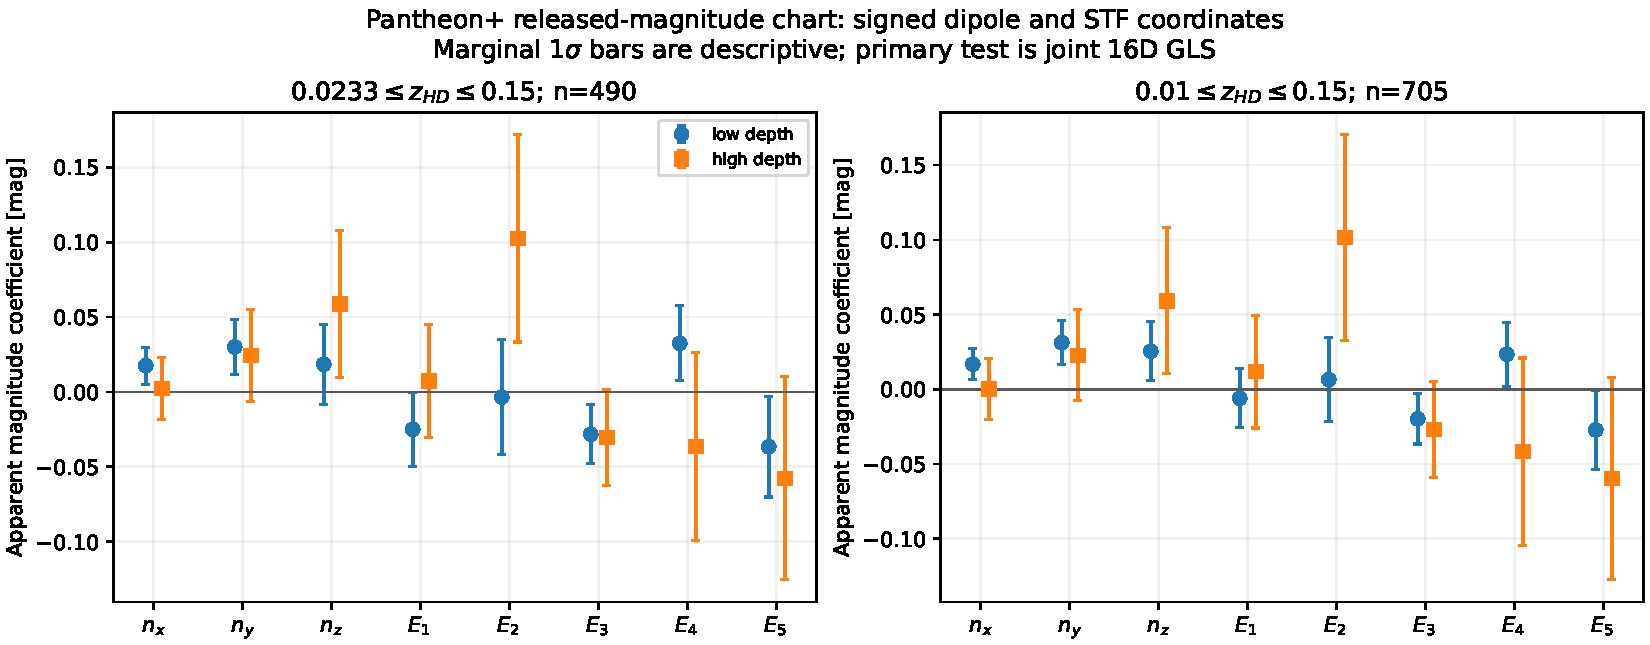
\includegraphics[width=1\textwidth,height=\textheight]{../../../OBSERVABLE_BRIDGE_RECONCILIATION_20261027/products/R36-08-PUBLIC-SN/PUBLIC_SN_SIGNED_COORDINATES.pdf}
\caption{Released-magnitude dipole and quadrupole coefficients in two
depth bins; displayed marginal errors accompany the retained full
covariance.}
\end{figure}

The consumed covariance subblocks are symmetric and positive definite.
The full release array fails the frozen symmetry tolerance outside their
support, so its validation does not extend beyond the selected blocks.
The primary cross-depth block contains 50,616 nonzero entries {[}E9{]}.
Treating the bins as independent would discard a measured part of the
adopted release covariance.

CF4 illustrates a different uncertainty mechanism. The exact retained
H03 operator acts on 35,970 selected groups. A stipulated common
Gaussian velocity field over
\(0.005\!\le k\le\!0.05\,h\,\mathrm{Mpc}^{-1}\), with the specified
independent source and method-offset terms, yields a conditional
covariance trace of 17.68057
\((\mathrm{km}\,\mathrm{s}^{-1}\,\mathrm{Mpc}^{-1})^2\) for the
36-coordinate \(R=5\,h^{-1}\mathrm{Mpc}\) result {[}E10{]}. This
transports a common physical field through the actual selected operator.
It does not add the inherited working variance again or turn an assumed
velocity law into an empirically calibrated selection model.

Optical transmission enters the physical interpretation through

\[
D_{L,r}(z,n)=\frac{cz}{\mathcal H_u(n)}
\exp\left[r_g(z,n)+\frac12\tau_r(z,n)\right].
\]

If \(|r_g|\le b_g\) and \(\tau_-\le\tau_r\le\tau_+\), the flux-based
\(H_F=cz/D_{L,r}\) gives

\[
H_Fe^{-b_g+\tau_-/2}\le\mathcal H_u(n)
\le H_Fe^{b_g+\tau_+/2}.
\]

This interval keeps finite-distance and attenuation assumptions visible.
For a calibrated matrix channel \(\mathcal A=D_L^{-2}\mathcal P\), its
input effect \(\mathcal A^*(I)\) constrains distance; relative channel
shape does not determine grey transmission.

For distance \(d_r=de^{\tau/2}\), the scalar CBL relation has the exact
correction

\[
C[d_r]=1+e^\tau(C[d]-1)
+\frac{d_r^2}{2c^2}(H^2\tau''+HH'\tau').
\]

In the flat synthetic control with \(\tau=0.2z\), the uncorrected
residual at \(z=1.5\) is \(-0.3498588\); exact correction returns zero
to roundoff. The declared opacity class instead gives the outer
geometric interval \([-0.3802306,0.0225]\) {[}E11{]}. This demonstrates
how a flux residual can coexist with flat geometry.

\begin{figure}
\centering
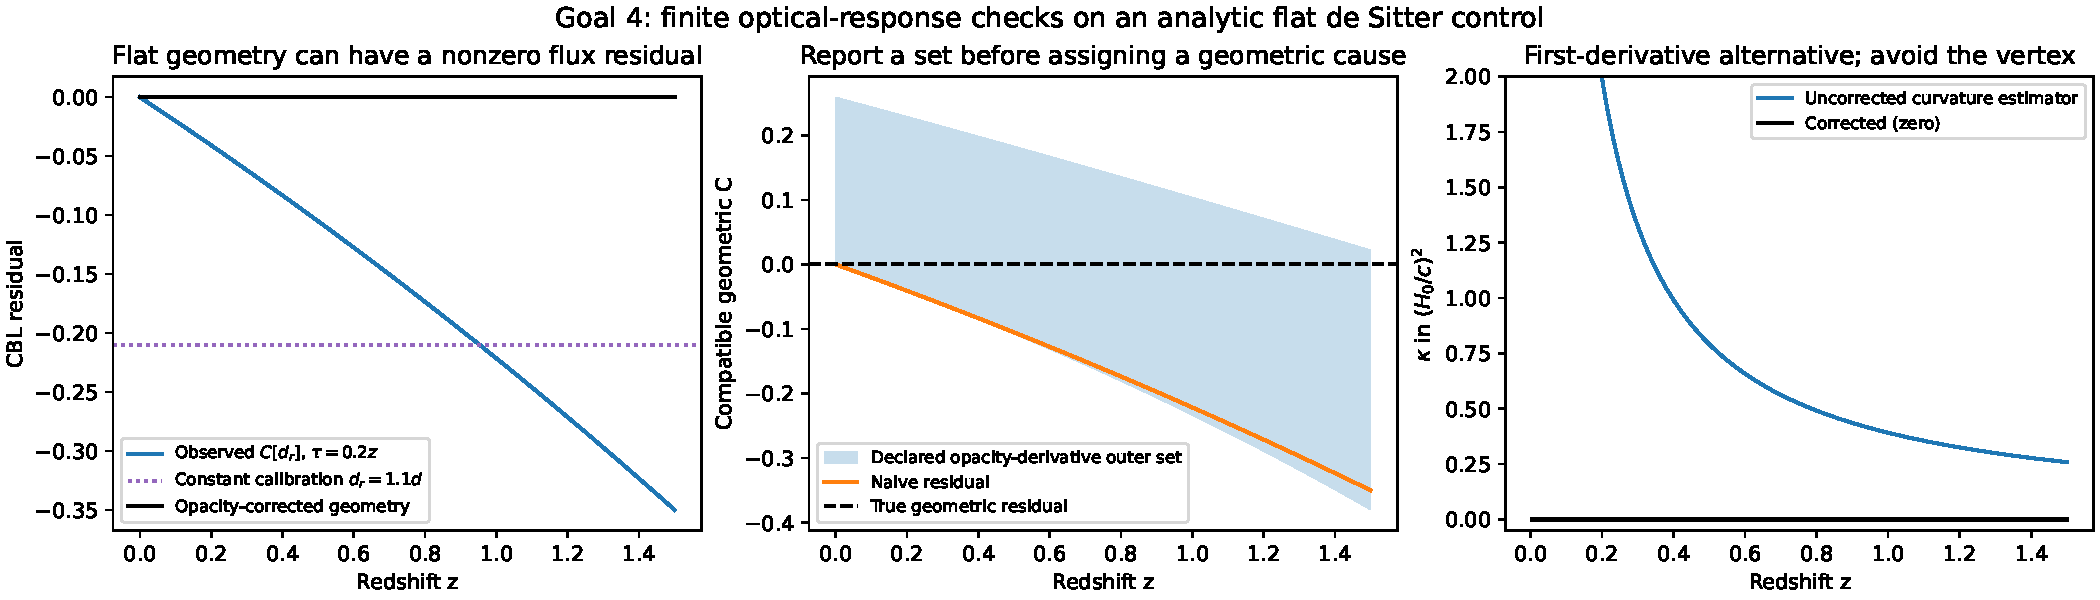
\includegraphics[width=1\textwidth,height=\textheight]{../../imports/four_goals/figures/goal4_cbl_opacity.pdf}
\caption{Flat-geometry optical control: attenuation-induced CBL
residual, its corrected value, and the permitted geometric interval.}
\end{figure}

The next empirical refinement uses a calibrated distance function and
independently qualified \(H(z)\) to test constancy of
\(\kappa(z)=[H^2d'^2/c^2-1]/d^2\), carrying opacity and calibration
through one joint event. The existing angular SN carrier supplies the
directional observation component; it does not by itself supply absolute
distance calibration or redshift derivatives.

\hypertarget{six-paper-crosswalk-and-current-boundaries}{%
\section{Six-paper crosswalk and current
boundaries}\label{six-paper-crosswalk-and-current-boundaries}}

The four physical chapters are a shared evidence base for the original
six paper topics. These rows describe reusable results, not completed
original paper acceptances.

\begin{longtable}[]{@{}
  >{\raggedright\arraybackslash}p{(\columnwidth - 6\tabcolsep) * \real{0.2500}}
  >{\raggedright\arraybackslash}p{(\columnwidth - 6\tabcolsep) * \real{0.2500}}
  >{\raggedright\arraybackslash}p{(\columnwidth - 6\tabcolsep) * \real{0.2500}}
  >{\raggedright\arraybackslash}p{(\columnwidth - 6\tabcolsep) * \real{0.2500}}@{}}
\toprule\noalign{}
\begin{minipage}[b]{\linewidth}\raggedright
Paper
\end{minipage} & \begin{minipage}[b]{\linewidth}\raggedright
Shared chapter(s)
\end{minipage} & \begin{minipage}[b]{\linewidth}\raggedright
Source-bound result used here
\end{minipage} & \begin{minipage}[b]{\linewidth}\raggedright
Remaining physical or publication gate
\end{minipage} \\
\midrule\noalign{}
\endhead
\bottomrule\noalign{}
\endlastfoot
P1 --- signed functionals and partial identification & 2, 4 & R32 H03
structured selected-law response and common-confidence method; finite
joint-remainder control & Parent selection and missing outcomes remain
separate from the selected-cohort law; no full physical functional
admission \\
P2 --- Planck morphology and anomalies & 1, 3 & R32 bounded-bandpass
methods; R36-05 common-input radiation comparison; optional first-48
total-map diagnostic below & R36-07 physical foreground radius, actual
MC100 qualification, matched observed/null processing and selection
accounting remain HOLD \\
P3 --- directional expansion & 4 & R36-01 exact H03 operator, R36-02
stipulated correlated field, R36-08 released SN signed coefficients & A
qualified joint physical response, calibration and redshift derivatives
are required for directional H(z,n) \\
P4 --- boosts, flow and global tilt & 2 & R32 finite response design and
R36-03 selected Gaia history response & External global-tilt history and
common-source physical comparisons remain required \\
P5 --- Bianchi observable equivalence & 3 & R32 finite algebraic region
and R36-10 conditional geometry images & All-m T/E/B native morphology
atlas, matched null/covariance and family-equivalence gates remain
HOLD \\
P6 --- kinematics & 1, 2, 4 & R32 optical inverse and R36-04
common-budget optical response & Source/frame, finite history and
derivative residuals must be supplied for physical sigma/omega/H
images \\
\end{longtable}

The late PR4/P2 preparation recorded by \texttt{UPSTREAM\_DELTA.json} is
a reviewed source/lifecycle preparation,
\textbf{PREPARED\_PENDING\_SOURCE\_QUALIFICATION}. It is not an approved
observational morphology result. The source-qualified R36-06 streaming
helper likewise does not establish an MC ensemble or promote the
original R36-07 foreground-budget task.

\hypertarget{auxiliary-first-48-processed-map-location-result}{%
\subsection{Auxiliary first-48 processed-map location
result}\label{auxiliary-first-48-processed-map-location-result}}

A separate independent review found a \textbf{scoped conditional
exploratory pass} for the first 48 Commander FULL005a processed-map
realizations, IDs 300--347. The saved carrier has 42 real E/B
coordinates, full 42-by-42 sample covariance, rank 42, and condition
number 58,283.91. Its total conditional mean norm is \textbf{0.07020
microkelvin}, with a conservative norm interval \textbf{{[}0, 0.82832{]}
microkelvin}. Under an \textbf{assumed iid multivariate Gaussian} law,
the fixed-sample Hotelling statistic is \textbf{T² = 3877.47}, its
stated critical value \textbf{1240.13}, and its nominal zero-mean F tail
\textbf{0.0025425}. A single 2,000-replicate Gaussian implementation
control covered \textbf{1886/2000 = 0.943}. These values describe the
selected processed outputs under that stipulated law. The iid law,
observed/MC conditional exchangeability, and selective coverage are
unestablished; after-exposure selection prevents a confirmatory null
claim. Total map location cannot be attributed uniquely to foregrounds,
the CMB parent, or processing bias. The review leaves \textbf{R36-07 and
all original-42 acceptances unchanged}. Its two nonblocking
routine-reuse findings concern exact zero displacement and an
independent positive basis fixture; neither changes this sealed
invocation. The review and sealed result are bound as A1 in the claim
map.

\hypertarget{evidence-map-and-reusable-source-definitions}{%
\section{Evidence map and reusable source
definitions}\label{evidence-map-and-reusable-source-definitions}}

Source baseline commit:
\texttt{bdead6a8f51282ca647224b460b0f65de085568b}; assembly checkout
HEAD: \texttt{cab89d25af52a1b978a4da8c11eecdc25bb22759}. The
accompanying \texttt{BASELINE\_REPORT.json} records exact repository
paths, numerical selectors, source hashes, figure bindings and scoped
qualification for each entry. No catalogue was refit for this report.

\begin{longtable}[]{@{}
  >{\raggedright\arraybackslash}p{(\columnwidth - 2\tabcolsep) * \real{0.5000}}
  >{\raggedright\arraybackslash}p{(\columnwidth - 2\tabcolsep) * \real{0.5000}}@{}}
\toprule\noalign{}
\begin{minipage}[b]{\linewidth}\raggedright
Evidence
\end{minipage} & \begin{minipage}[b]{\linewidth}\raggedright
Bound result
\end{minipage} \\
\midrule\noalign{}
\endhead
\bottomrule\noalign{}
\endlastfoot
E1 & Saved Gaussian compression and common-family likelihood
comparison \\
E2 & Joint physical remainder and fixed-law coverage experiment \\
E3 & R36 radiation response, target coverage and moment truncation \\
E4 & Joint Thomson/shear carrier and polarized collision omission \\
E5 & R36 source-level optical inverse and shared octupole budget \\
E6 & Detector/angular rank and frame-spin quotient \\
E7 & R36 selected-sample electric-quadrupole history response \\
E8 & R36 spatial Ricci witnesses and fixed-Q chirality radius \\
E9 & R36 released SN angular coefficients and selected covariance \\
E10 & R36 correlated CF4 covariance through the source-bound operator \\
E11 & Exact opacity correction and finite CBL control \\
E12 & Finite fibre-count information and calibration experiment \\
A1 & Independently reviewed first-48 total processed-map diagnostic
under assumed iid Gaussian law \\
\end{longtable}

The physical response conventions follow the primary derivations
identified in the retained source notes: Challinor's covariant polarized
multipoles, Marcori et al.'s observer/source proper-motion response, the
Gauss relations in relativistic cosmology, and the Clarkson--Bassett--Lu
distance/expansion consistency relation. Their application here is
specified by the source frames, response maps and uncertainty laws
above.

\begin{itemize}
\tightlist
\item
  A. Challinor, \emph{Microwave background polarization in cosmological
  models}, Phys. Rev.~D 62, 043004 (2000),
  \href{https://arxiv.org/abs/astro-ph/9911481}{astro-ph/9911481}.
\item
  O. H. Marcori et al., \emph{Direction and redshift drifts for general
  observers and their applications in cosmology}, Phys. Rev.~D 98,
  023517 (2018), \href{https://arxiv.org/abs/1805.12121}{1805.12121}.
\item
  C. G. Tsagas, A. Challinor and R. Maartens, \emph{Relativistic
  cosmology and large-scale structure}, Physics Reports 465, 61--147
  (2008), \href{https://arxiv.org/abs/0705.4397}{0705.4397}.
\item
  C. Clarkson, B. A. Bassett and T. H.-C. Lu, \emph{A general test of
  the Copernican Principle}, Phys. Rev.~Lett. 101, 011301 (2008),
  \href{https://arxiv.org/abs/0712.3457}{0712.3457}.
\end{itemize}

\end{document}
